
\section*{Problema P7.10}

\renewcommand*\thesection{7.10}
\numberwithin{equation}{section}

\begin{center}
    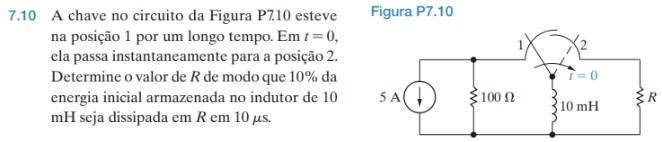
\includegraphics[scale=1.0]{P7.10.jpg}
\end{center}


Vamos entender primeiramente como estava o estado inicial antes da chave comutar ($t < 0$). \\
Em regime permanente de corrente contínua, o indutor se comporta como um curto-circuito. Assim,
toda a corrente $i = 5A$ da fonte passava sobre ele, e a queda de tensão no resistor era zero. Portanto,

\[ i_L(0) = 5 \un{A} \]

Quando a chave comuta, temos a seguinte equação de malha

\[ L\diff{i}{t} + iR = 0 \]

Que é uma EDO cuja solução já é conhecida 

\begin{equation}\label{eq:7.10.1}
    i(t) = i(0)e^{-\frac{R}{L}t}
\end{equation}

Com constante de tempo $\tau = \frac{R}{L}$.

A energia no indutor é dada por 

\begin{equation}\label{eq:7.10.2}
    E(t) = \frac{1}{2}L[i(t)]^2
\end{equation}

Substituindo \eqref{eq:7.10.1} em \eqref{eq:7.10.2}, temos

\[ E(t) = \frac{1}{2}L[i(0)e^{-\frac{R}{L}t}]^2 \]

Isolando $R$, temos 
 
\[ -\frac{2t}{L}R = \ln\left(\frac{2E(t)}{Li_0^2}\right) \]

\[ R = -\frac{L}{2t} \ln\left(\frac{2E(t)}{Li_0^2}\right) \]

Para que o resistor $R$ dissipe $10\%$ da energia inicial no indutor, temos o indutor deve ter $90\%$ da energia inicial no instante
$t$, ou seja, 

\[ E(t) = \frac{9}{10}E_0  \]

Substituindo na expressão de $R$,

\[ R = -\frac{L}{2t} \ln\left(\frac{2\frac{9}{10}E_0}{Li_0^2}\right) \]

Note que $E_0 = \frac{1}{2}Li_0^2$. Logo,

\[ R = -\frac{L}{2t} \ln\left(\frac{2\frac{9}{10}\frac{1}{2}Li_0^2}{Li_0^2}\right) \]

\[ R = -\frac{L}{2t} \ln\left(\frac{9}{10}\right) \]

Assim, para que essa dissipação de energia ocorra no instante $t = 10\;\mu s$, temos 

\[ \boxed{R = 52.68 \;\Omega}  \]



